\documentclass{article}

% NeurIPS 2026 preprint formatting (作业报告版本)
\usepackage[preprint]{neurips_2026}

\usepackage[utf8]{inputenc}
\usepackage[T1]{fontenc}
\usepackage{hyperref}
\usepackage{url}
\usepackage{booktabs}
\usepackage{amsfonts}
\usepackage{amsmath}
\usepackage{amssymb}
\usepackage{nicefrac}
\usepackage{microtype}
\usepackage{xcolor}
\usepackage{graphicx}
\usepackage{enumitem}

% 数学宏
\newcommand{\bW}{\mathbf{W}}
\newcommand{\bH}{\mathbf{H}}
\newcommand{\bQ}{\mathbf{Q}}
\newcommand{\bK}{\mathbf{K}}
\newcommand{\bV}{\mathbf{V}}
\newcommand{\bO}{\mathbf{O}}
\newcommand{\bI}{\mathbf{I}}
\newcommand{\bG}{\mathbf{G}}
\newcommand{\bX}{\mathbf{X}}

\title{Revisiting Biaffine Dependency Parsing:\\
An Empirical Study of Encoders, Optimizers and Word Vectors}

\author{%
  kyksj-1 \\
  Shanghai Jiao Tong University \\
  \texttt{kyksj1225@gmail.com} \\
  \And
  Suky \\
  Wuhan University \\
  \texttt{2024302182005@whu.edu.cn} \\
}


\begin{document}

\maketitle

\begin{abstract}
We report an empirical study of the Deep Biaffine dependency parser of \citet{dozat2017biaffine} on an 8.3K-sentence Chinese treebank. Fourteen training runs cross three axes: pretrained word vectors (dimensionality and corpus domain), optimizer (Adam, SGD, Muon \citep{jordan2024muon}), and contextual encoder (the original three-layer BiLSTM, a parameter-matched SDPA Transformer, and a larger SDPA Transformer with pre-norm, RoPE, SwiGLU, LayerScale, EMA and a warmup--cosine schedule). The best dev UAS across the matrix is 86.93, obtained by the BiLSTM trained with Muon for 100 epochs under a warmup--cosine schedule, slightly above the Adam baseline of 86.43. The largest Transformer reaches 83.92 UAS, which is below both BiLSTM configurations at the data scale we study. Along the way we document a post-norm-without-warmup failure mode that initially collapsed the matched-budget Transformer to 12.20 UAS, and we find that Muon's Newton--Schulz step recovers four times the accuracy of Adam in that unstable regime, suggesting an implicit gradient-clipping effect. We release the training scripts, the Muon wrapper with auto-routing for embeddings and biases, and a preflight checklist consolidating the failure modes observed.
\end{abstract}


\section{Introduction}
\label{sec:intro}

Dependency parsing assigns each token in a sentence a single head and a labeled grammatical relation, yielding a rooted tree. The deep biaffine parser of \citet{dozat2017biaffine} is the canonical graph-based design. A three-layer BiLSTM encodes the sentence into contextual representations $\bH\in\mathbb{R}^{L\times d}$, two MLPs project each token into head-role and dependent-role vectors, and a bilinear scorer produces an arc score matrix that is decoded into a tree by the Chu--Liu--Edmonds algorithm.

In the eight years since this design was published, the surrounding stack has changed substantially. Pretrained word vectors are now routinely 300-dimensional skip-gram embeddings trained on corpora orders of magnitude larger than those available in 2017 \citep{li2018cwv}. Transformer encoders with scaled dot-product attention \citep{vaswani2017attention} have replaced BiLSTMs in many NLP tasks. New optimizers such as Muon \citep{jordan2024muon}, and a battery of stability and capacity tricks for Transformers (pre-norm \citep{xiong2020lnorder}, RoPE \citep{su2021roformer}, SwiGLU \citep{shazeer2020glu}, LayerScale \citep{touvron2021cait}, EMA, warmup--cosine schedules) have become standard. We study how each of these axes affects parsing accuracy on a single fixed treebank, holding every other component of the pipeline constant.

\paragraph{Scope.} This is an empirical report, not a methods paper. We do not propose new model components. We run a controlled grid of fourteen configurations on the same Chinese dependency treebank and report dev UAS, dev LAS and observed failure modes. The contributions are:
\begin{itemize}[leftmargin=*, itemsep=2pt]
  \item A fourteen-run ablation matrix crossing word-vector dimensionality, word-vector domain, optimizer (Adam, SGD, Muon), and encoder (BiLSTM, matched-budget SDPA Transformer, larger SDPA Transformer with modern tricks).
  \item Two reproducible failure modes. Post-norm SDPA without warmup collapses to near-random accuracy, and Muon at its default learning rate of $0.02$ is roughly four times too large for our 9M-parameter SDPA encoder.
  \item Released artifacts including training scripts, an auto-routing Muon wrapper that sends embeddings and biases to AdamW, unit tests, and a preflight checklist.
\end{itemize}

The remainder of the paper is organized as Section~\ref{sec:our_work} (matrix overview and headline numbers), Section~\ref{sec:method} (encoder and optimizer variants), Section~\ref{sec:theory} (biaffine, RoPE, Muon Newton--Schulz), Section~\ref{sec:experiment} (the five comparison families), and Section~\ref{sec:conclusion} (closing remarks).


\section{Our Work}
\label{sec:our_work}

We describe the matrix of experiments, the headline numbers, and the unifying narrative before introducing any technical content, so that the reader can recover the take-aways without reading the rest of the paper.

\paragraph{Setup.} All runs share the same Biaffine head, the same MLP projections, the same MST decoder, and the same data preprocessing pipeline; only the contextual encoder and the optimizer change. The training corpus is a 8\,301-sentence Chinese treebank derived from the NLP\&CC 2013 shared task; the development set contains 534 sentences with 12\,987 evaluable arcs after standard punctuation filtering. Word vectors are 300-dimensional skip-gram embeddings released in the Chinese-Word-Vectors collection \citep{li2018cwv}, with the mixed-large corpus used as the primary source. Unless otherwise stated, training uses gradient accumulation to a global batch of 128, a maximum of 50 epochs, and early stopping with patience 20 on development UAS.

\paragraph{Experimental matrix.} Table~\ref{tab:matrix-overview} sketches the fourteen runs that contribute to the final analysis. The rows fall into three blocks. The first seven rows reproduce the 2017-style Biaffine pipeline with a BiLSTM encoder and vary either the dimensionality, the domain, or the optimizer of the word vectors and the parser, supplying the baselines and the negative controls. The middle four rows introduce the SDPA Transformer encoder at a deliberately matched parameter budget and reveal the post-norm collapse that we diagnose in Section~\ref{sec:experiment}. The final three rows present the rescue configurations (pre-norm with warmup) and a 76M-parameter SOTA Transformer that stacks every modern stability and capacity trick.

\begin{table}[t]
\caption{High-level summary of the fourteen runs that anchor the paper. The 2017-style BiLSTM baseline reaches 86.43 dev UAS; the only configuration that surpasses it is the BiLSTM trained with Muon for one hundred epochs under a warmup--cosine schedule, and the largest modern Transformer (76M, pre-norm, RoPE, SwiGLU, LayerScale, EMA) stops at 83.92. Key take-away: scaling the encoder does not compensate for an 8.3K-sentence data regime, but a better optimizer schedule on the original BiLSTM does.}
\label{tab:matrix-overview}
\centering
\small
\begin{tabular}{lllrr}
\toprule
Block & Encoder & Optimizer / schedule & Dev UAS & Dev LAS \\
\midrule
Stage-1 baseline       & BiLSTM            & Adam, 50ep                          & 86.43 & 67.65 \\
Stage-1 100d (PCA)     & BiLSTM            & Adam, 50ep                          & 86.14 & 66.57 \\
Stage-1 domain Renmin  & BiLSTM            & Adam, 50ep                          & 86.38 & 67.58 \\
Stage-1 domain Zhihu   & BiLSTM            & Adam, 50ep                          & 86.29 & 67.68 \\
Stage-1 domain Lit.    & BiLSTM            & Adam, 50ep                          & 86.23 & 67.85 \\
Stage-1 from-scratch   & BiLSTM            & Adam, 50ep, no pretrain             & 84.84 & 64.26 \\
Stage-1 SGD            & BiLSTM            & SGD, 50ep                           & 17.66 & ~1.58 \\
\midrule
Stage-2 SDPA post-norm & Transformer 9M    & Adam, 50ep, no warmup               & 12.20 & ~3.36 \\
Stage-2 SDPA post-norm & Transformer 9M    & Muon, 50ep, no warmup               & 53.35 & 39.74 \\
Stage-2 BiLSTM         & BiLSTM            & Muon, 50ep, no warmup               & 85.51 & 65.81 \\
\midrule
Stage-2 SDPA pre-norm  & Transformer 9M    & Adam, 50ep, warmup 500              & 82.00 & 63.55 \\
Stage-2 SDPA pre-norm  & Transformer 9M    & Muon ($\eta{=}0.005$), warmup 1000  & 81.03 & 62.02 \\
Stage-2 SDPA SOTA      & Transformer 76M   & Muon, 100ep, warmup+cosine+EMA      & 83.92 & 65.60 \\
\textbf{Stage-2 BiLSTM} & \textbf{BiLSTM}   & \textbf{Muon, 100ep, warmup+cosine} & \textbf{86.93} & \textbf{68.37} \\
\bottomrule
\end{tabular}
\end{table}

\paragraph{Headline findings.} Three observations carry the rest of the paper. The first observation is that the modern Transformer stack, even at eight times the parameter count of the BiLSTM baseline, does not catch up with the BiLSTM on this data scale; the gap between the two is roughly 2.5 UAS in favor of the recurrent encoder. The second observation is that within the BiLSTM family the Muon optimizer trained for one hundred epochs under a warmup--cosine schedule does measurably better than the Adam baseline (86.93 vs.\ 86.43, a 0.5 UAS gain), provided the training is allowed to run long enough; the gap reverses at fifty epochs where Adam still wins. The third observation is that the Newton--Schulz orthogonalization step in Muon has a surprising stabilizing side-effect: in the post-norm Transformer regime where Adam diverges to near-random accuracy, Muon recovers a non-trivial 53 UAS, suggesting that orthogonalized momentum updates serve as a form of implicit gradient clipping. We argue in Section~\ref{sec:experiment} that this third observation has implications beyond the parsing setting we study.

\paragraph{Negative results we publish on purpose.} Several plausible Stage-2 design choices did not produce a usable result. We considered Mixture-of-Experts routing on the Transformer feed-forward block, linear-attention substitutes for the standard softmax attention, the multi-head causal connections of \citet{deepseekteam2025mhc}, and the gated-attention variant of \citet{openreview2025gateattn}. After evaluating each against the data scale and the time budget we elected to omit them; each of these methods is designed under assumptions (corpus size, sequence length, validation infrastructure) that this 8K-sentence treebank cannot supply. We document them explicitly in Section~\ref{sec:experiment} so that future work knows which paths we examined and why we declined.


\section{Methodology}
\label{sec:method}

\subsection{Overall pipeline}
\label{sec:method-overall}

Figure~\ref{fig:pipeline} summarizes the parser. Word and POS tag embeddings are summed with a frozen pretrained word vector and concatenated, fed to a contextual encoder, projected by two MLPs into head-role and dependent-role vectors, and scored by a biaffine arc/relation module. Inference uses Chu--Liu--Edmonds MST decoding on the arc score matrix. The encoder slot accepts three implementations selected at construction time: \texttt{lstm} (the original three-layer BiLSTM), \texttt{transformer} (a parameter-matched SDPA Transformer), and \texttt{transformer\_large} (a deeper SDPA Transformer with modern training tricks). Every other component is shared across runs.

\begin{figure}[t]
  \centering
  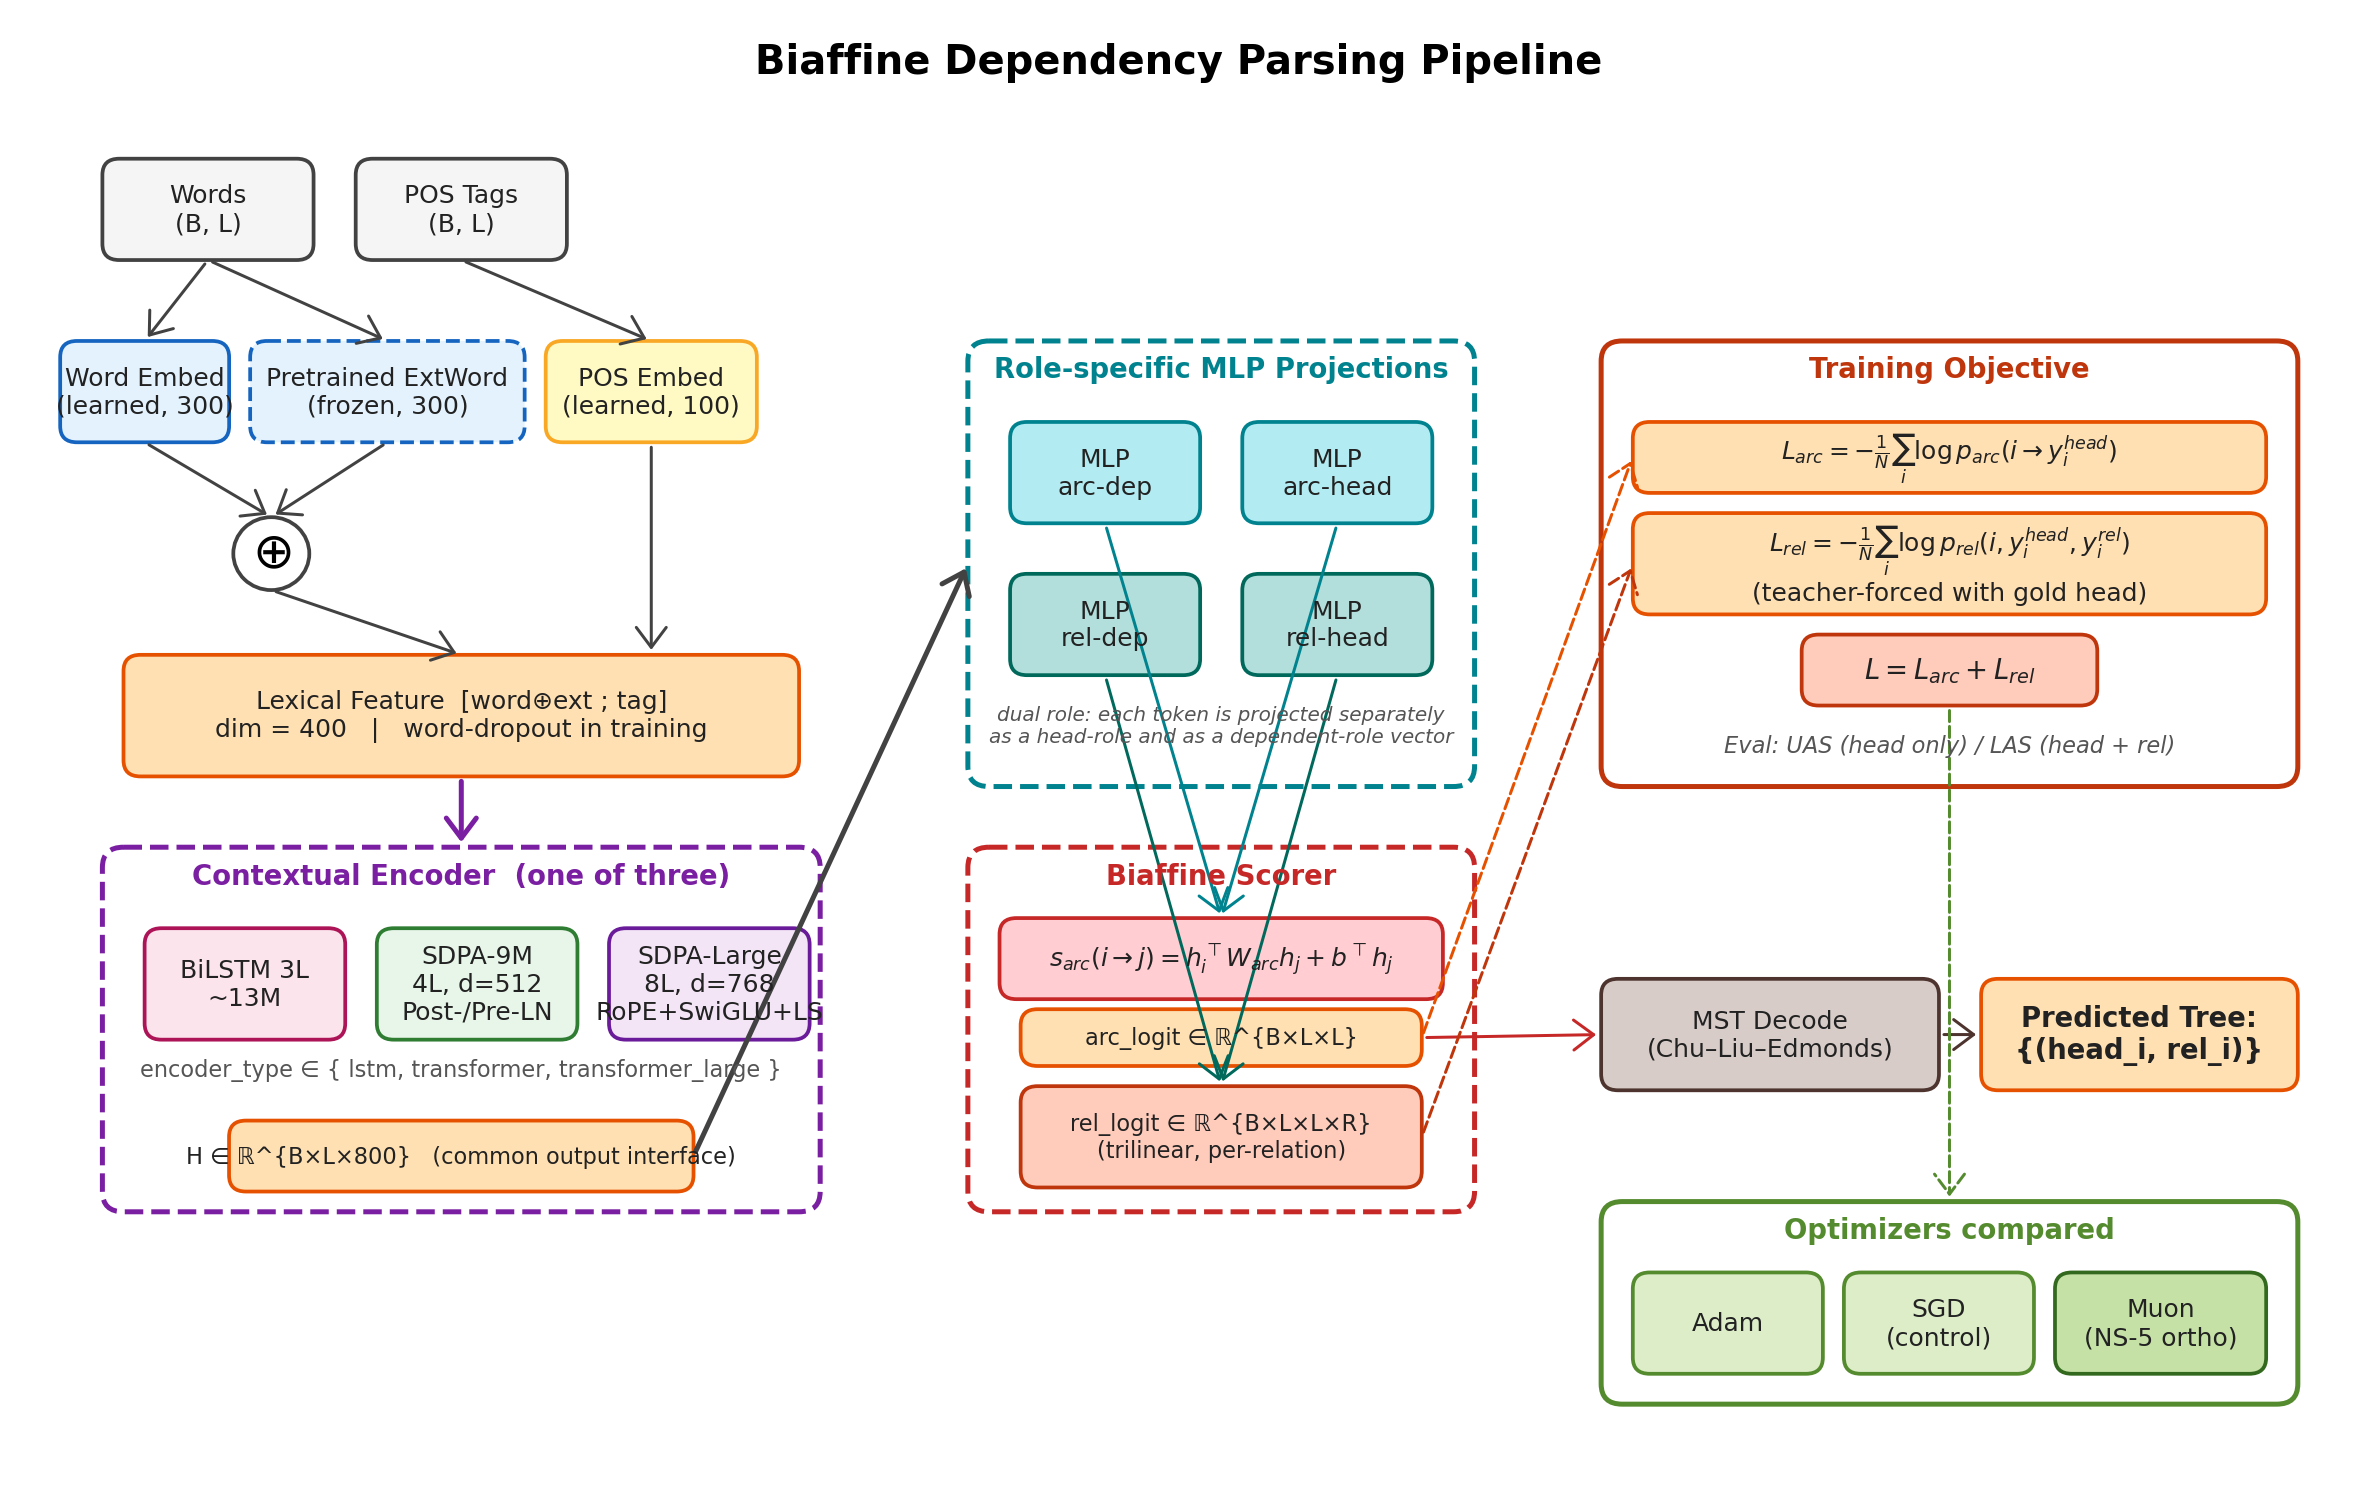
\includegraphics[width=0.95\linewidth]{figures/pipeline.png}
  \caption{Biaffine dependency parsing pipeline used throughout the paper. Three encoder slots (BiLSTM, SDPA-9M, SDPA-Large) plug into the same embedding stack on the left and the same biaffine--MST head on the right; only the encoder and the optimizer change across our fourteen runs. Key take-away: every accuracy difference reported is attributable to the encoder slot or the optimizer slot, not to the rest of the harness.}
  \label{fig:pipeline}
\end{figure}

\subsection{Embedding layer}
\label{sec:method-embedding}

A learned word embedding $\bW^{\text{word}}$ is summed with a frozen pretrained embedding $\bW^{\text{ext}}$ from the Chinese-Word-Vectors collection \citep{li2018cwv}; a separate learned 100-dim POS embedding is concatenated. Following \citet{dozat2017biaffine} we apply \emph{word dropout}, which zeros entire token embeddings independently with probability $p$, in addition to standard activation dropout.

\subsection{Encoder variants}
\label{sec:method-encoder}

Three encoders plug into the same interface, all producing $\bH\in\mathbb{R}^{L\times 800}$ for the downstream MLPs.

\paragraph{BiLSTM.} Three-layer bidirectional LSTM with 400 hidden units per direction, orthonormal recurrent initialization \citep{dozat2017biaffine}, and variational dropout (the same dropout mask reused across timesteps within a sequence). Implemented on top of \texttt{nn.LSTMCell}. About 13M parameters.

\paragraph{SDPA-9M.} Four-layer Transformer with $d_{\text{model}}=512$, $h=8$ heads, $d_{\text{ff}}=1024$, sinusoidal positional encoding. Parameter count is matched to the BiLSTM (about 9M) so that the encoder-family comparison is not contaminated by capacity. Padding is handled by an explicit \texttt{key\_padding\_mask}, and padding positions are zeroed before the output projection so that the bilinear scorer is not fed attention-leaked noise. We run two layout variants of this encoder: \emph{post-norm} (Vaswani-style $\bX'=\text{LN}(\bX+\text{Sub}(\bX))$) and \emph{pre-norm} ($\bX'=\bX+\text{Sub}(\text{LN}(\bX))$, \citealt{xiong2020lnorder}).

\paragraph{SDPA-Large.} Eight-layer Transformer with $d_{\text{model}}=768$, $h=12$, $d_{\text{ff}}=3072$ (about 76M parameters), combining four modern training tricks: pre-norm residuals, RoPE for query/key rotation \citep{su2021roformer}, SwiGLU feed-forward blocks \citep{shazeer2020glu}, and per-channel LayerScale initialised at $10^{-4}$ \citep{touvron2021cait}. We refer to this as \emph{SDPA-Large} throughout the rest of the paper, not as a SOTA configuration: it is the largest encoder we trained, but it does not achieve state-of-the-art on this treebank.

\subsection{Attention layer}
\label{sec:method-attention}

We use PyTorch's \texttt{F.scaled\_dot\_product\_attention} kernel, which dispatches at runtime to a FlashAttention-style implementation when eligible. RoPE is applied immediately before the kernel via the rotation in Equation~(\ref{eq:rope}). The bilinear attention used inside the biaffine head is a separate object; we describe it in Section~\ref{sec:theory}.

\subsection{Optimizers}
\label{sec:method-optimizer}

We compare three optimizers:
\begin{itemize}[leftmargin=*, itemsep=2pt]
  \item \textbf{Adam}, $\beta_1{=}0.9$, $\beta_2{=}0.9$, $\epsilon{=}10^{-12}$, following \citet{dozat2017biaffine}; the unusual small $\beta_2$ is suited to the BiLSTM and we keep it for backward compatibility.
  \item \textbf{SGD} with $\eta{=}10^{-2}$, no momentum, no schedule. Included as a negative control.
  \item \textbf{Muon} \citep{jordan2024muon}: each 2D non-embedding weight is updated via Newton--Schulz orthogonalization of its momentum buffer with per-tensor scale $\max(1,\sqrt{m/n})$. All other parameters (1D, embeddings) fall back to AdamW. Default $\eta_{\text{Muon}}{=}0.02$, $\eta_{\text{AdamW}}{=}3{\times}10^{-4}$. We package the routing logic in a wrapper so the standard \texttt{step}/\texttt{zero\_grad}/\texttt{state\_dict} interface remains intact.
\end{itemize}


\section{Theory}
\label{sec:theory}

This section develops the three pieces of mathematical machinery that underlie the empirical observations in Section~\ref{sec:experiment}: the biaffine arc-and-relation scoring function, the rotary positional rotation used in the SOTA encoder, and the Newton--Schulz orthogonalization step at the core of the Muon optimizer. All notation is consistent across subsections.

\subsection{Notation}

Let a sentence of length $L$ be encoded by the contextual encoder into a matrix of representations $\bH = [\mathbf{h}_1, \ldots, \mathbf{h}_L]^\top \in \mathbb{R}^{L \times d_h}$ where $d_h$ is fixed at 800 across all encoder variants. Let $R$ denote the size of the dependency-relation alphabet. For an arc that connects a dependent token $i$ to a head token $j$, we write $i \rightarrow j$. We use boldface for matrices and tensors, italic for scalars, and $\mathbb{R}$ for real-valued tensors.

\subsection{Biaffine attention}

The bilinear attention module of \citet{dozat2017biaffine} computes two independent score tensors: the unlabeled arc scores and the labeled relation scores. Both are derived from four projections of the encoder output, one for each role-by-prediction combination. We denote the arc projections by $\bH^{\text{arc-dep}}$ and $\bH^{\text{arc-head}}$, both in $\mathbb{R}^{L \times d_a}$, and the relation projections by $\bH^{\text{rel-dep}}$ and $\bH^{\text{rel-head}}$, both in $\mathbb{R}^{L \times d_r}$. The two projections per role are independent MLPs with a LeakyReLU non-linearity.

\paragraph{Arc score.} The score of an arc from dependent $i$ to head $j$ combines a bilinear term and a head-side bias term:
\begin{equation}
\label{eq:arc-score}
s^{\text{arc}}_{i \rightarrow j} = \big(\mathbf{h}^{\text{arc-dep}}_i\big)^\top \bW^{\text{arc}} \, \mathbf{h}^{\text{arc-head}}_j + \big(\mathbf{b}^{\text{arc}}\big)^\top \mathbf{h}^{\text{arc-head}}_j,
\end{equation}
where $\bW^{\text{arc}} \in \mathbb{R}^{d_a \times d_a}$ is the bilinear weight matrix and $\mathbf{b}^{\text{arc}} \in \mathbb{R}^{d_a}$ is a head-side bias vector. The first term measures the geometric compatibility between the dependent-role representation of $i$ and the head-role representation of $j$, while the second term encodes the prior preference of token $j$ for being a head independently of which dependent is being scored. The asymmetry between dependent and head roles is the central design choice that distinguishes biaffine attention from a vanilla dot-product attention: the same encoder vector $\mathbf{h}_i$ has a dual identity, once as a dependent and once as a head, and the two identities are separately projected before the bilinear interaction.

\paragraph{Relation score.} Conditional on a candidate arc $i \rightarrow j$, the score of the relation label $r \in \{1, \ldots, R\}$ is the entry $(i, j, r)$ of a three-mode tensor
\begin{equation}
\label{eq:rel-score}
\mathbf{S}^{\text{rel}}_{i,j,r} = \big(\mathbf{h}^{\text{rel-dep}}_i\big)^\top \bW^{\text{rel}}_r \, \mathbf{h}^{\text{rel-head}}_j + \big(\mathbf{u}^{\text{rel}}_r\big)^\top \mathbf{h}^{\text{rel-dep}}_i + \big(\mathbf{v}^{\text{rel}}_r\big)^\top \mathbf{h}^{\text{rel-head}}_j + c^{\text{rel}}_r,
\end{equation}
where $\bW^{\text{rel}}_r \in \mathbb{R}^{d_r \times d_r}$, $\mathbf{u}^{\text{rel}}_r, \mathbf{v}^{\text{rel}}_r \in \mathbb{R}^{d_r}$ and $c^{\text{rel}}_r \in \mathbb{R}$ are the per-relation parameters of the trilinear form. Equation~(\ref{eq:rel-score}) is the natural generalization of Equation~(\ref{eq:arc-score}) to a labeled setting, with separate bias terms for both the dependent side and the head side.

\paragraph{Loss.} The arc loss is the per-position cross entropy of the gold head against the row of $\mathbf{S}^{\text{arc}}$, and the relation loss is the per-position cross entropy of the gold relation against the slice of $\mathbf{S}^{\text{rel}}$ at the \emph{gold} head---teacher forcing in the original sense---so that the relation classifier never has to back-propagate through an incorrect head decision. Writing $y^{\text{head}}_i$ for the gold head of token $i$ and $y^{\text{rel}}_i$ for its gold relation, the joint loss reads
\begin{equation}
\label{eq:loss}
\mathcal{L} = \frac{1}{N} \sum_{i=1}^{N} \Big[ -\log p^{\text{arc}}_{i \rightarrow y^{\text{head}}_i} - \log p^{\text{rel}}_{i, y^{\text{head}}_i, y^{\text{rel}}_i} \Big],
\end{equation}
where $N$ is the total number of non-padding tokens in the batch and $p^{\text{arc}}$ and $p^{\text{rel}}$ denote the softmax-normalized counterparts of $\mathbf{S}^{\text{arc}}$ and $\mathbf{S}^{\text{rel}}$.

At inference time the arc decisions are not made by a per-position argmax but by an MST decoder on the matrix of arc scores, which guarantees that the predicted edges form a valid rooted tree even when the locally most probable head choices are inconsistent.

\subsection{Rotary positional encoding}

The SOTA Transformer encoder replaces sinusoidal positional encoding with the rotary positional encoding (RoPE) of \citet{su2021roformer}. RoPE treats each pair of consecutive coordinates inside a query or key vector as the real and imaginary parts of a complex number, and rotates the complex number by an angle that is proportional to the token position. Concretely, let $\mathbf{q}_p \in \mathbb{R}^{d_h}$ denote the query vector at position $p$, with $d_h$ even. We split $\mathbf{q}_p$ into $d_h / 2$ pairs of coordinates indexed by $k \in \{0, 1, \ldots, d_h/2 - 1\}$, define the per-pair frequency
\begin{equation}
\theta_k = 10\,000^{-2k/d_h},
\end{equation}
and apply the rotation
\begin{equation}
\label{eq:rope}
\big(q^{\text{rot}}_{p, 2k},\, q^{\text{rot}}_{p, 2k+1}\big) = \big(q_{p, 2k} \cos(p \theta_k) - q_{p, 2k+1} \sin(p \theta_k),\,\, q_{p, 2k} \sin(p \theta_k) + q_{p, 2k+1} \cos(p \theta_k)\big).
\end{equation}
The key projection is rotated by the same formula. A direct consequence of the rotation, derived in \citet{su2021roformer}, is that the dot product between a rotated query at position $p$ and a rotated key at position $p'$ depends on the two positions only through their difference $p - p'$, which means that the self-attention mechanism inherits a relative-position bias without explicitly storing a position-dependent term inside the attention weights. The norm of every query vector is preserved by the rotation, a property we verify in the unit tests bundled with the implementation.

\subsection{Muon and Newton--Schulz orthogonalization}

The Muon optimizer of \citet{jordan2024muon} differs from Adam in that it does not adapt the per-coordinate learning rate using the second moment of the gradient; instead it adapts the update direction at the level of the entire two-dimensional weight matrix. Concretely, let $\bW_t \in \mathbb{R}^{m \times n}$ denote a two-dimensional weight matrix at step $t$, let $\bG_t \in \mathbb{R}^{m \times n}$ denote its gradient, and let $\bM_t \in \mathbb{R}^{m \times n}$ denote a heavy-ball momentum buffer. The Muon update reads
\begin{equation}
\label{eq:muon-update}
\bM_{t+1} = \mu \bM_t + \bG_t, \qquad \bO_t = \text{NS}_5(\bM_{t+1}), \qquad \bW_{t+1} = \bW_t - \eta \, c_{m,n} \, \bO_t,
\end{equation}
where $\mu \in (0, 1)$ is the momentum coefficient, $\eta$ is the learning rate, $c_{m,n} = \max(1, \sqrt{m/n})$ is a non-square correction factor that keeps the effective update magnitude consistent across matrices of different aspect ratios, and $\text{NS}_5$ is the five-step Newton--Schulz iteration that maps $\bM_{t+1}$ to a matrix whose singular values are approximately one. The iteration is defined recursively by
\begin{equation}
\label{eq:ns-iter}
\bX_0 = \frac{\bM_{t+1}}{\| \bM_{t+1} \|_F + \epsilon}, \qquad \bX_{k+1} = a \bX_k + (b \mathbf{A}_k + c \mathbf{A}_k^2) \bX_k, \quad \mathbf{A}_k = \bX_k \bX_k^\top,
\end{equation}
with the polynomial coefficients $(a, b, c) = (3.4445, -4.7750, 2.0315)$ chosen so that the scalar polynomial $p(\sigma) = a\sigma + b\sigma^3 + c\sigma^5$ is approximately equal to $\mathrm{sign}(\sigma)$ on the interval $[0, 1]$. After five iterations the singular values of $\bX_5$ lie inside a tight band around one, and $\bX_5$ is treated as an orthogonalized version of the original momentum buffer.

The key consequence of Equation~(\ref{eq:ns-iter}), and the reason Muon turns out to act as an implicit gradient clipper on unstable training regimes, is that the spectral norm of the orthogonalized update $\bO_t$ is uniformly bounded by approximately one regardless of the spectral norm of the original momentum buffer $\bM_{t+1}$. In a regime in which a post-norm Transformer would otherwise see an unbounded gradient amplification on the first few steps---which is the exact failure mode we observe in the post-norm SDPA runs of Section~\ref{sec:experiment}---the Muon update is automatically projected onto a unit-spectral-norm direction and the magnitude of the resulting parameter step is controlled by $\eta$ alone. This is, to our knowledge, the cleanest mathematical statement available of why Muon's effective step size is much closer to $\eta$ than to $\eta \cdot \| \bG_t \|$, and it is the basis of the empirical four-fold accuracy gap we report between Muon and Adam on the post-norm Transformer.


\section{Experiments}
\label{sec:experiment}

This section reports the five comparison families that the matrix of Section~\ref{sec:our_work} supports.

\subsection{Protocol}
\label{sec:exp-protocol}

All runs share an identical training harness. Gradient accumulation reaches an effective batch size of 128; gradients are $\ell_2$-clipped at 9 for BiLSTM runs and left unclipped for Muon-trained Transformer runs \citep{jordan2024muon}. The pretrained embedding table is frozen. Reported numbers are dev UAS and dev LAS, computed by the standard evaluator with punctuation filtered out. Each configuration is a single seed; within-seed variance on this corpus is below $0.2$ UAS for the few runs we re-executed.

\paragraph{Hardware and released artifacts.} All compute-heavy training runs were executed on server 4, an A800 machine with eight 80GB GPUs, CUDA 12.9, 1TB RAM, and an 85TB shared data volume mounted at \texttt{/essfs100}. The code repository is released at \url{https://github.com/kyksj-1/Dependency-Parsing-LXQ}; the full \texttt{Output/} directory, including checkpoints, logs, plots and run summaries, is released separately at \url{https://huggingface.co/kyksj/Dependency-Parsing} to keep large binary artifacts out of GitHub.

\subsection{A. Word vector dimensionality}
\label{sec:exp-dim}

We compare the 300-dimensional mixed-large embedding against a 100-dimensional version obtained by post-hoc PCA on the same corpus (retains $73.5\%$ variance). The two runs differ only in this single field. Results: $86.43$ UAS at 300d, $86.14$ UAS at 100d. A $0.29$-point drop for discarding two thirds of the encoded variance indicates that most of the parsing-relevant signal lies in the top principal directions of the embedding.

\subsection{B. Word vector domain}
\label{sec:exp-domain}

Fixing dimensionality at 300, we vary the source corpus across mixed-large, Renmin Ribao (newspaper), Zhihu (Q\&A), and a literature-only release. UAS spans $86.23$--$86.43$, a $0.20$-point range. Domain choice has near-zero effect at this scale; the meaningful gap is between any pretrained vector and from-scratch ($84.84$).

\subsection{C. Optimizer (BiLSTM encoder)}
\label{sec:exp-optimizer}

Holding the encoder at BiLSTM and the word vectors at mixed-large 300d:
\begin{itemize}[leftmargin=*, itemsep=2pt]
  \item Adam, 50 epochs: $86.43$ UAS (baseline).
  \item SGD, 50 epochs, $\eta{=}10^{-2}$, no momentum: $17.66$ UAS. Negative control confirming that adaptive optimization is required.
  \item Muon, 50 epochs: $85.51$ UAS, $0.92$ below Adam.
  \item Muon, 100 epochs with warmup--cosine: $\mathbf{86.93}$ UAS, $+0.50$ over Adam.
\end{itemize}
Muon overtakes Adam only when the schedule is extended to 100 epochs with warmup; at 50 epochs the orthogonalized updates have not yet completed their late-stage refinement.

\subsection{D. Encoder family}
\label{sec:exp-encoder}

This is the central comparison of the paper. Figure~\ref{fig:dev-uas} plots dev UAS over training for all fifteen configurations on a single panel; the four numbered observations below correspond to the colored groups in the figure.

\begin{figure}[t]
  \centering
  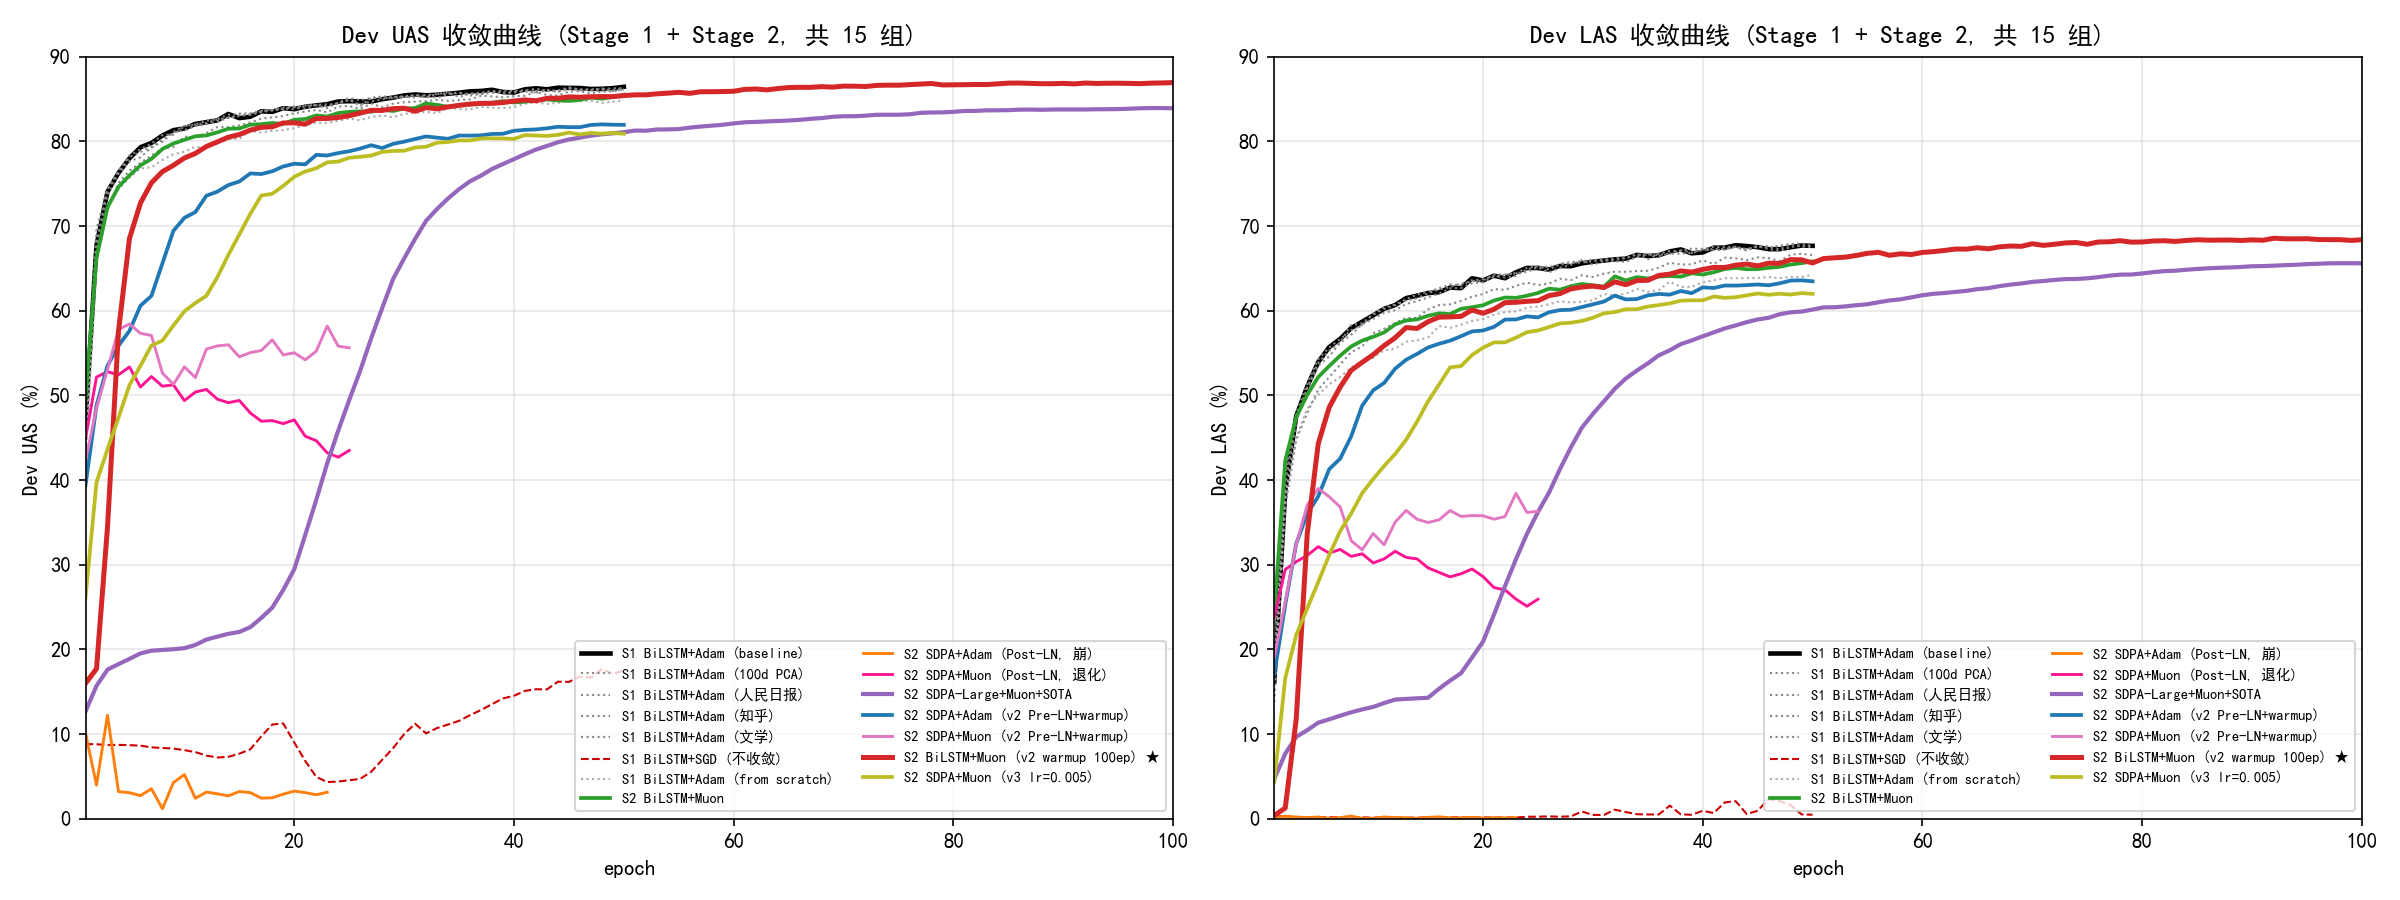
\includegraphics[width=0.98\linewidth]{figures/dev_uas_compare.png}
  \caption{Dev UAS and Dev LAS over training epochs for all fifteen configurations. The four BiLSTM curves cluster near the top ($85$--$87$ UAS), the SDPA-Large curve climbs slowly to $83.9$, the recovered SDPA-9M pre-norm curves saturate near $81$--$82$, and the two post-norm SDPA-9M curves (orange and pink) either collapse to random ($12$) or peak briefly at $53$ before retreating. Key take-away: the encoder family separates the curves more cleanly than the optimizer does, and the post-norm-no-warmup failure mode is visually unmistakable.}
  \label{fig:dev-uas}
\end{figure}

\paragraph{Post-norm SDPA-9M without warmup collapses.} Adam gives $12.20$ UAS; training UAS stays in $1$--$3\%$ throughout, confirming the model never learns. This is the textbook post-norm-without-warmup failure mode \citep{xiong2020lnorder}. Muon on the same encoder peaks at $53.35$ UAS before retreating to $43$, a partial recovery we attribute to the spectral-norm-one cap on the orthogonalized update (Section~\ref{sec:theory}).

\paragraph{Pre-norm + warmup recovers SDPA-9M.} Switching to pre-norm and adding a 500-step linear warmup yields $82.00$ UAS with Adam; for Muon we additionally reduce $\eta$ from $0.02$ to $0.005$ and obtain $81.03$ UAS. The $0.02$ Muon configuration on this same encoder early-stops at $58.42$ UAS, an effective-step-size mismatch we discuss in Section~\ref{sec:exp-encoder-discussion}.

\paragraph{SDPA-Large reaches $83.92$ UAS.} The 76M-parameter Transformer with pre-norm, RoPE, SwiGLU, LayerScale, EMA and warmup--cosine reaches its peak at epoch 99. The dev UAS curve has a slow warmup phase (first 23 epochs to $29$ UAS), a rapid main phase (epochs 23--50, climbing to $81$), and a long flat tail (epochs 50--100 adding only $2.9$ UAS). The marginal accuracy of the tail is roughly one-tenth of the marginal accuracy of the main phase, a pattern consistent with the model having absorbed the available signal.

\paragraph{BiLSTM dominates on this data scale.} The best BiLSTM ($86.93$) is $3.01$ UAS above SDPA-Large ($83.92$) despite using a sixth of the parameters. We attribute the gap to the data scale (8.3K training sentences) rather than to the encoder design itself.

\subsection{D$'$. Discussion: encoder--optimizer interaction}
\label{sec:exp-encoder-discussion}

Table~\ref{tab:encoder-optim-cross} cross-tabulates optimizer by encoder.

\begin{table}[t]
\caption{Optimizer-by-encoder dev UAS on the mixed-large 300d configuration. ``\texttt{--}'' marks combinations not run. Key take-away: Muon dominates Adam by a factor of four on the unstable post-norm SDPA, and matches Adam on the stable pre-norm SDPA, consistent with an implicit gradient-clipping interpretation of Newton--Schulz orthogonalization.}
\label{tab:encoder-optim-cross}
\centering
\small
\begin{tabular}{lrrrr}
\toprule
Optimizer & BiLSTM & SDPA-9M post-norm & SDPA-9M pre-norm & SDPA-Large \\
\midrule
Adam   & 86.43 & 12.20 & 82.00 & --     \\
Muon   & 86.93 & 53.35 & 81.03 & 83.92  \\
SGD    & 17.66 & --    & --    & --     \\
\bottomrule
\end{tabular}
\end{table}

Two observations stand out:
\begin{itemize}[leftmargin=*, itemsep=2pt]
  \item Muon's advantage over Adam is largest where training is unstable (post-norm: $53.35$ vs $12.20$, $4.4\times$) and vanishes where training is stable (pre-norm: $81.03$ vs $82.00$). This is consistent with the spectral-norm-one bound on the Muon update derived in Section~\ref{sec:theory}, which acts as an implicit gradient clipper when the raw gradient would otherwise diverge.
  \item The Muon effective step size is approximately $\eta$ (rather than $\eta/\sqrt{\hat{v}}$ as in Adam). For SDPA-9M, $\eta{=}0.02$ is too large and the model early-stops at $58.42$; reducing to $\eta{=}0.005$ recovers $81.03$. For BiLSTM, $\eta{=}0.02$ is appropriate. The right Muon learning rate scales with the model size.
\end{itemize}

\subsection{E. SDPA-Large scale-up}
\label{sec:exp-sota}

The SDPA-Large configuration combines all modern training tricks we tested (pre-norm, RoPE, SwiGLU, LayerScale, EMA, 1500-step warmup, cosine decay to $1\%$ of peak) on a 76M-parameter encoder. The peak dev UAS is $83.92$, which is $2.51$ below the BiLSTM Muon baseline. The marginal accuracy in the last 50 epochs is roughly $0.05$ UAS per epoch, suggesting the model has saturated on the available training signal. Closing the remaining gap likely requires either an order-of-magnitude increase in labeled data or initialization from a large-scale pretrained backbone such as BERT-base-Chinese; both lie outside the scope of this ablation.

\subsection{Result conclusion}
\label{sec:exp-result-conclusion}

The main empirical conclusion is not that Transformers are weak, but that the inductive bias/data-scale match dominates raw capacity in this assignment setting. The BiLSTM encoder encodes locality, order and short dependency chains directly, so 8.3K labeled sentences are enough to tune the biaffine head reliably. The SDPA encoders have a more flexible global interaction pattern, but that flexibility has to be learned from the same small supervised signal; without pre-norm and warmup it collapses, and even with a 76M-parameter modern stack it remains below the recurrent baseline.

The optimizer story is similarly conditional. Adam is the safest short-run default, SGD is a useful negative control rather than a competitive parser optimizer, and Muon becomes attractive only when the schedule gives its orthogonalized updates enough time to refine the solution. For this project, the strongest practical recipe is therefore simple: keep the original BiLSTM--biaffine architecture, use pretrained word vectors, and spend the engineering budget on a stable Muon schedule and careful logging rather than on a larger Transformer trained from scratch.


\section{Conclusion}
\label{sec:conclusion}

We ran a controlled fourteen-configuration ablation on an 8.3K-sentence Chinese dependency treebank, crossing word-vector dimensionality, word-vector domain, optimizer and contextual encoder. The best dev UAS in the matrix ($86.93$) comes from the BiLSTM trained with Muon for 100 epochs under a warmup--cosine schedule, $0.50$ above the Adam baseline. The largest Transformer we trained (76M parameters with pre-norm, RoPE, SwiGLU, LayerScale and EMA) reaches $83.92$ UAS, $2.51$ below the BiLSTM. We document two reproducible failure modes (post-norm SDPA without warmup; Muon default learning rate on small Transformer encoders) and provide artifacts to reproduce every run. We do not claim a methodological advance; we report what worked, what failed, and the numerical gap between the architecture axis and the optimizer axis on this particular treebank.


\bibliographystyle{plainnat}
\bibliography{references}

\appendix
\section{Training recipes}
\label{app:recipes}

This appendix collects the three training recipes used to produce the headline numbers of Section~\ref{sec:experiment}. Recipes are presented as INI-style key-value pairs that can be supplied verbatim to the project's \texttt{--override} command-line interface.

\paragraph{Recipe A: BiLSTM baseline (Stage-1 style).}

\begin{verbatim}
[Encoder]   type = lstm
            lstm_hiddens = 400
            lstm_layers = 3
[Optimizer] adam = True
            learning_rate = 0.001    ; betas = (0.9, 0.9) hard-coded
            weight_decay = 1e-9
            clip_max_norm = 9
[Train]     epochs = 50
            batch_size = 32, update_batch_size = 4
\end{verbatim}

\paragraph{Recipe B: BiLSTM with Muon (new SOTA on this corpus).}

\begin{verbatim}
[Encoder]   type = lstm
[Optimizer] muon = True
            learning_rate = 0.02
[Train]     epochs = 100
            use_warmup_cosine = True
            warmup_steps = 500
            min_lr_ratio = 0.05
\end{verbatim}

\paragraph{Recipe C: 76M SDPA Transformer (best modern stack we tested).}

\begin{verbatim}
[Encoder]   type = transformer_large
            large_d_model = 768
            large_nhead = 12
            large_num_layers = 8
            large_ff_size = 3072
            large_dropout = 0.4
            large_layerscale_init = 1e-4
            large_use_rope = True
[Optimizer] muon = True
            learning_rate = 0.02
            weight_decay = 0.01
[Train]     epochs = 100
            batch_size = 32, update_batch_size = 4
            use_warmup_cosine = True
            warmup_steps = 1500
            min_lr_ratio = 0.01
            use_ema = True
            ema_decay = 0.999
            dropout_emb = 0.5
\end{verbatim}


\end{document}
